\documentclass[
  11pt,
  letterpaper,
   addpoints,
   answers
  ]{exam}

\usepackage{../exercise-preamble}
\usepackage{float}
\usepackage{pgfplots}
\pgfplotsset{compat=1.18}
% TikZ libraries needed for `right=.. of ..` and coordinate math
\usetikzlibrary{positioning,calc,arrows,arrows.meta}
% Alias de seguridad por si se escribe 'ikzstyle' por error
\let\ikzstyle\tikzstyle

% Comando para títulos de modo con líneas al ancho del texto
\newlength{\rulelength}
\newcommand{\modtitle}[1]{%
  \settowidth{\rulelength}{\textbf{#1}}%
  \par\addvspace{6pt}\noindent%
  \begin{tabular}{@{}l@{}}
    \rule{\rulelength}{0.5pt}\\[3pt]%
    \textbf{#1}\\[3pt]%
    \rule{\rulelength}{0.5pt}%
  \end{tabular}%
  \par\addvspace{8pt}%
}

\begin{document}

% Configuración del encabezado usando comandos de la clase exam
\pagestyle{headandfoot}
\extraheadheight{0.5in}
\firstpageheader{\textit{Microondas}}{}{EL7029}
\runningheader{\textit{Microondas}}{}{EL7029}
\firstpagefooter{}{\thepage}{}
\runningfooter{}{\thepage}{}
\headrule

% Numeración de página
\pagenumbering{arabic}

% Portada
\begin{center}
    \vspace*{1cm}
    
    % Logo superior
    
\includegraphics[width=0.5\textwidth]{../fcfm_die}
    
    \vspace{2cm}
    
    % Líneas decorativas superiores
    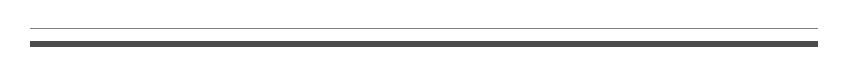
\begin{tikzpicture}
        \draw[line width=2pt, black!70] (0,0) -- (10,0);
        \draw[line width=0.5pt, black!50] (0,0.2) -- (10,0.2);
    \end{tikzpicture}
    
    \vspace{1cm}
    
    % Título principal
    {\fontsize{28}{34}\selectfont\bfseries 
   Microondas}
    
    \vspace{0.5cm}
    
    {\Large\textbf{EL7029}}
    
    \vspace{0.3cm}
    
    {\large Guías de Ondas}
    
    \vspace{1cm}
    
    % Líneas decorativas inferiores
    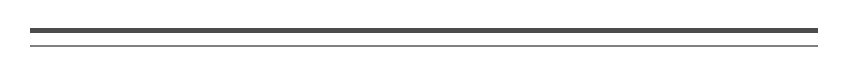
\begin{tikzpicture}
        \draw[line width=0.5pt, black!50] (0,0) -- (10,0);
        \draw[line width=2pt, black!70] (0,0.2) -- (10,0.2);
    \end{tikzpicture}
    
    \vspace{1.5cm}
    
    % Subtítulo
    {\LARGE\itshape Auxiliar 2}
    
    \vspace{1cm}

    % Cuadro semestre y profesores
    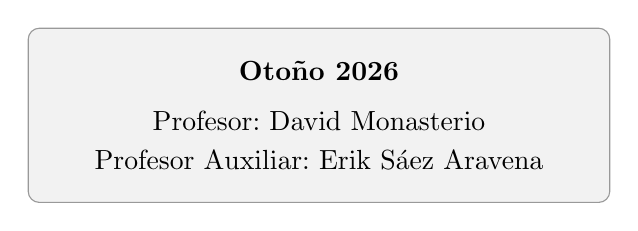
\begin{tikzpicture}
        \node[draw=black!40, fill=black!5, rounded corners=4pt,
              inner xsep=24pt, inner ysep=12pt, align=center] {
            \textbf{Otoño 2026}\\[6pt]
            Profesor:\ David Monasterio\\[2pt]
            Profesor Auxiliar:\ Erik Sáez Aravena
        };
    \end{tikzpicture}

    \vfill

    \vspace{1cm}
    
\end{center}

\newpage

\begin{questions}
    %%%%%%%%%%%%%%%%%%%%%%%%%%%
\question \textbf{Soluciones generales TEM/TE/TM y especialización a guía rectangular.}

\begin{parts}

%-------------------- (a) FIGURA GENERAL + MODOS --------------------
\part Considere las estructuras de la Fig.~\ref{fig:waveguide_general}: línea de dos conductores y guía cerrada, ambas uniformes en $z$,
con medio $(\epsilon,\mu)$ y propagación $e^{-j\beta z}$.
Clasifique los modos en TEM, TE y TM según $E_z$ y $H_z$, y obtenga las expresiones generales de los campos transversales
a partir de las componentes longitudinales usando Maxwell en fasores.

\begin{figure}[H]
    \centering
    
\includegraphics[width=0.6\textwidth]{Auxiliar_2_1}
    \caption{(a) Línea de transmisión general de dos conductores. (b) Guía cerrada de un solo conductor.}
    \label{fig:waveguide_general}
\end{figure}
\begin{solution}
\modtitle{Ecuaciones generales}
Dado que buscamos definir los campos transversales a partir de los longitudinales, conviene escribir los campos de la siguiente manera:
\begin{equation}
\mathbf{E}(x,y,z)=\big[\mathbf{e}(x,y)+\hat{\mathbf z}\,e_z(x,y)\big]\,e^{-j\beta z},
\qquad
\mathbf{H}(x,y,z)=\big[\mathbf{h}(x,y)+\hat{\mathbf z}\,h_z(x,y)\big]\,e^{-j\beta z},
\end{equation}
Es de interés separar los campos en componentes transversales y longitudinales respecto al eje de propagación $z$. En esta notación,
\begin{align*}
\mathbf{e}(x,y)= \hat{\mathbf x}\,e_x+\hat{\mathbf y}\,e_y,\qquad
\mathbf{h}(x,y)= \hat{\mathbf x}\,h_x+\hat{\mathbf y}\,h_y
\end{align*}
son los campos transversales. Se omite la dependencia temporal $e^{j\omega t}$ dado que asumimos régimen permanente. Por otro lado, recordemos que las ecuaciones de Maxwell en fasores
para un medio homogéneo, lineal e isótropo sin fuentes libres son:
\begin{equation}
\nabla\times \mathbf{E}=-j\omega\mu\,\mathbf{H},
\qquad
\nabla\times \mathbf{H}=j\omega\epsilon\,\mathbf{E}.
\end{equation}
Dado que las estructuras son uniformes en $z$ y se asume propagación $e^{-j\beta z}$, el operador $\partial/\partial z \to -j\beta$.
\newpage
\noindent
\begin{minipage}[t]{0.485\linewidth}
\textbf{(i) Ecuaciones desde $\nabla\times \mathbf{E}=-j\omega\mu\,\mathbf{H}$.}\\[-2pt]
Aplicando el rotacional:
\begin{align*}
\nabla\times\mathbf{E} =
\begin{vmatrix}
\hat{\mathbf{x}} & \hat{\mathbf{y}} & \hat{\mathbf{z}} \\[4pt]
\partial_x & \partial_y & -j\beta \\[4pt]
E_x & E_y & E_z
\end{vmatrix}
= -j\omega\mu\,\mathbf{H},
\end{align*}
se obtiene:
\begin{align}
\frac{\partial E_z}{\partial y}+j\beta E_y&=-j\omega\mu H_x,
\label{eq:3a}\\
-j\beta E_x-\frac{\partial E_z}{\partial x}&=-j\omega\mu H_y,
\label{eq:3b}\\
\frac{\partial E_y}{\partial x}-\frac{\partial E_x}{\partial y}&=-j\omega\mu H_z.
\label{eq:3c}
\end{align}
\end{minipage}%
\hfill
\begin{minipage}[t]{0.485\linewidth}
\textbf{(ii) Ecuaciones desde $\nabla\times \mathbf{H}=j\omega\epsilon\,\mathbf{E}$.}\\[-2pt]
Análogamente:
\begin{align*}
\nabla\times\mathbf{H} =
\begin{vmatrix}
\hat{\mathbf{x}} & \hat{\mathbf{y}} & \hat{\mathbf{z}} \\[4pt]
\partial_x & \partial_y & -j\beta \\[4pt]
H_x & H_y & H_z
\end{vmatrix}
= j\omega\epsilon\,\mathbf{E},
\end{align*}
se obtiene:
\begin{align}
\frac{\partial H_z}{\partial y}+j\beta H_y&=j\omega\epsilon E_x,
\label{eq:4a}\\
-j\beta H_x-\frac{\partial H_z}{\partial x}&=j\omega\epsilon E_y,
\label{eq:4b}\\
\frac{\partial H_y}{\partial x}-\frac{\partial H_x}{\partial y}&=j\omega\epsilon E_z.
\label{eq:4c}
\end{align}
\end{minipage}

\vspace{6pt}
A partir de \eqref{eq:3a}--\eqref{eq:4c}, se desea eliminar $E_x,E_y,H_x,H_y$ para expresar los cuatro campos transversales en función de
$E_z$ y $H_z$ (esto es útil pues luego se analizan modos TE con $E_z=0$ y TM con $H_z=0$). Para ello definimos:
\begin{equation}
k^2 \triangleq \omega^2\mu\epsilon,
\qquad
k_c^2 \triangleq k^2-\beta^2.
\label{eq:defkc}
\end{equation}

\noindent
\begin{minipage}[t]{0.47\linewidth}
\textbf{(iii) Obtención de $E_y$ y $H_x$}\\
Para esto utilizaremos las ecuaciones \eqref{eq:3a} y \eqref{eq:4b}.
\begin{align}
H_x&=-\frac{1}{j\omega\mu}\left(\frac{\partial E_z}{\partial y}+j\beta E_y\right).
\label{eq:Hx_from3a}
\end{align}
Sustituyendo \eqref{eq:Hx_from3a} en \eqref{eq:4b} y expandiendo:
\begin{align*}
-j\beta H_x-\frac{\partial H_z}{\partial x}&=j\omega\epsilon E_y,\\
\frac{\beta}{\omega\mu}\frac{\partial E_z}{\partial y}+\frac{j\beta^2}{\omega\mu}E_y-\frac{\partial H_z}{\partial x}
&=j\omega\epsilon E_y,\\
-\frac{j}{\omega\mu}\underbrace{(\omega^2\mu\epsilon-\beta^2)}_{k_c^2}E_y
&=-\frac{\beta}{\omega\mu}\frac{\partial E_z}{\partial y}+\frac{\partial H_z}{\partial x}.
\end{align*}
Por tanto:
\begin{align}
E_y&=\frac{j}{k_c^2}\left(-\beta\frac{\partial E_z}{\partial y}+\omega\mu\frac{\partial H_z}{\partial x}\right).
\label{eq:Ey_final}
\end{align}
Reemplazando \eqref{eq:Ey_final} en \eqref{eq:Hx_from3a}:
\begin{align}
H_x&=\frac{j}{k_c^2}\left(\omega\epsilon\frac{\partial E_z}{\partial y}-\beta\frac{\partial H_z}{\partial x}\right).
\label{eq:Hx_final}
\end{align}
\end{minipage}%
\hfill
\begin{minipage}[t]{0.49\linewidth}
\textbf{(iv) Obtención de $E_x$ y $H_y$}.\\
Para esto utilizaremos las ecuaciones \eqref{eq:3b} y \eqref{eq:4a}.
\begin{align}
H_y&=\frac{1}{j\omega\mu}\left(j\beta E_x+\frac{\partial E_z}{\partial x}\right).
\label{eq:Hy_from3b}
\end{align}
Sustituyendo \eqref{eq:Hy_from3b} en \eqref{eq:4a} y expandiendo:
\begin{align*}
\frac{\partial H_z}{\partial y}+j\beta H_y&=j\omega\epsilon E_x,\\
\frac{\partial H_z}{\partial y}+\frac{j\beta^2}{\omega\mu}E_x+\frac{\beta}{\omega\mu}\frac{\partial E_z}{\partial x}
&=j\omega\epsilon E_x,\\
-\frac{j}{\omega\mu}\underbrace{(\omega^2\mu\epsilon-\beta^2)}_{k_c^2}E_x
&=-\frac{\partial H_z}{\partial y}-\frac{\beta}{\omega\mu}\frac{\partial E_z}{\partial x}.
\end{align*}
Por tanto:
\begin{align}
E_x&=-\frac{j}{k_c^2}\left(\beta\frac{\partial E_z}{\partial x}+\omega\mu\frac{\partial H_z}{\partial y}\right).
\label{eq:Ex_final}
\end{align}
Reemplazando \eqref{eq:Ex_final} en \eqref{eq:Hy_from3b}:
\begin{align}
H_y&=-\frac{j}{k_c^2}\left(\omega\epsilon\frac{\partial E_z}{\partial x}+\beta\frac{\partial H_z}{\partial y}\right).
\label{eq:Hy_final}
\end{align}
\end{minipage}
De esta manera se han obtenido las expresiones generales de los campos transversales en función de los campos longitudinales:
\newpage
\noindent
\begin{minipage}[t]{0.485\linewidth}
\textbf{Campos magnéticos transversales:}\\[-2pt]
\begin{align}
H_x &= \frac{j}{k_c^2}\!\left(\omega\epsilon\frac{\partial E_z}{\partial y}-\beta\frac{\partial H_z}{\partial x}\right),\\[4pt]
H_y &= -\frac{j}{k_c^2}\!\left(\omega\epsilon\frac{\partial E_z}{\partial x}+\beta\frac{\partial H_z}{\partial y}\right).
\end{align}
\end{minipage}%
\hfill
\begin{minipage}[t]{0.485\linewidth}
\textbf{Campos eléctricos transversales:}\\[-2pt]
\begin{align}
E_x &= -\frac{j}{k_c^2}\!\left(\beta\frac{\partial E_z}{\partial x}+\omega\mu\frac{\partial H_z}{\partial y}\right),\\[4pt]
E_y &= \frac{j}{k_c^2}\!\left(-\beta\frac{\partial E_z}{\partial y}+\omega\mu\frac{\partial H_z}{\partial x}\right).
\end{align}
\end{minipage}
\modtitle{Caso ondas TEM}
En el caso TEM se cumple
\[
E_z=0,\qquad H_z=0,
\]
por lo que, al sustituir directamente en las expresiones generales para los campos transversales (en función de $E_z$ y $H_z$), los numeradores se anulan. Por esta razón se vuelve al conjunto de ecuaciones escalares obtenidas de Maxwell con dependencia $e^{-j\beta z}$, ecuaciones \eqref{eq:3a}--\eqref{eq:4c}, e imponemos $E_z=H_z=0$ (modo TEM), cada una implica:
\begin{align}
\frac{\partial E_z}{\partial y}+j\beta E_y&=-j\omega\mu H_x
&&\Longrightarrow&& j\beta E_y=-j\omega\mu H_x,
\label{eq:TEM_red1}\\
-j\beta E_x-\frac{\partial E_z}{\partial x}&=-j\omega\mu H_y
&&\Longrightarrow&& -j\beta E_x=-j\omega\mu H_y,
\label{eq:TEM_red2}\\
\frac{\partial H_z}{\partial y}+j\beta H_y&=j\omega\epsilon E_x
&&\Longrightarrow&& j\beta H_y=j\omega\epsilon E_x,
\label{eq:TEM_red3}\\
-j\beta H_x-\frac{\partial H_z}{\partial x}&=j\omega\epsilon E_y
&&\Longrightarrow&& -j\beta H_x=j\omega\epsilon E_y.
\label{eq:TEM_red4}
\end{align}
Usando \eqref{eq:TEM_red1} y \eqref{eq:TEM_red4} eliminamos $H_x$.
De \eqref{eq:TEM_red1}:
\begin{equation}
H_x=-\frac{\beta}{\omega\mu}\,E_y.
\label{eq:Hx_in_terms_Ey}
\end{equation}
Sustituyendo \eqref{eq:Hx_in_terms_Ey} en \eqref{eq:TEM_red4}:
\begin{equation}
-j\beta\left(-\frac{\beta}{\omega\mu}E_y\right)=j\omega\epsilon E_y
\quad\Longrightarrow\quad
j\frac{\beta^2}{\omega\mu}E_y=j\omega\epsilon E_y.
\end{equation}
Cancelando el factor común $jE_y$ (para un modo no trivial $E_y\neq 0$):
\begin{equation}
\frac{\beta^2}{\omega\mu}=\omega\epsilon
\quad\Longrightarrow\quad
\beta^2=\omega^2\mu\epsilon.
\end{equation}
Por tanto,
\begin{equation}
\beta=\omega\sqrt{\mu\epsilon}=k,
\end{equation}
Para el caso de las ondas TEM la constante de propagación axial es la misma que en una onda plana en el medio. Retomando lo siguiente:
\[
\nabla\times\mathbf{E}=-j\omega\mu\,\mathbf{H},\qquad \nabla\times\mathbf{H}=j\omega\epsilon\,\mathbf{E}.
\]
Tomando el rotacional de la primera ecuación y sustituyendo la segunda:
\begin{align*}
\nabla\times(\nabla\times\mathbf{E})
&=-j\omega\mu\,(\nabla\times\mathbf{H})
=-j\omega\mu\,(j\omega\epsilon\,\mathbf{E})
=\omega^2\mu\epsilon\,\mathbf{E}.
\end{align*}
Usando la identidad vectorial $\nabla\times(\nabla\times\mathbf{E})=\nabla(\nabla\cdot\mathbf{E})-\nabla^2\mathbf{E}$
y la ley de Gauss $\nabla\cdot\mathbf{E}=0$ (sin cargas libres):
\begin{align*}
-\nabla^2\mathbf{E}=\omega^2\mu\epsilon\,\mathbf{E}
\quad\Longrightarrow\quad
\nabla^2\mathbf{E}+k^2\mathbf{E}=\mathbf{0},\qquad k^2=\omega^2\mu\epsilon.
\end{align*}
Componente a componente, cada coordenada cartesiana satisface la ecuación de Helmholtz escalar.
En particular:
\begin{equation}
\left(\frac{\partial^2}{\partial x^2}+\frac{\partial^2}{\partial y^2}+\frac{\partial^2}{\partial z^2}+k^2\right)E_x=0,
\label{eq:Helmholtz_Ex}
\end{equation}
Con dependencia $e^{-j\beta z}$, se tiene
\[
\frac{\partial^2 E_x}{\partial z^2}=(-j\beta)^2 E_x=-\beta^2 E_x.
\]
Sustituyendo en \eqref{eq:Helmholtz_Ex}:
\begin{equation}
\left(\frac{\partial^2}{\partial x^2}+\frac{\partial^2}{\partial y^2}-\beta^2+k^2\right)E_x=0.
\end{equation}
Pero en TEM se cumple $\beta^2=k^2$, por lo que resulta:
\begin{equation}
\left(\frac{\partial^2}{\partial x^2}+\frac{\partial^2}{\partial y^2}\right)E_x=0.
\label{eq:Laplace_Ex}
\end{equation}
Un resultado análogo se obtiene para $E_y$, por lo que el campo eléctrico transversal $\mathbf{e}(x,y)$ satisface una ecuación de Laplace en la sección:
\begin{equation}
\nabla_t^2\,\mathbf{e}(x,y)=\mathbf{0},
\qquad
\nabla_t^2\triangleq \frac{\partial^2}{\partial x^2}+\frac{\partial^2}{\partial y^2}.
\label{eq:Laplace_et}
\end{equation}
Las líneas de $\mathbf{E}_t$ comienzan en un conductor y terminan en el otro, y el potencial transversal satisface Laplace (no hay fuentes libres en el dieléctrico).

\modtitle{TM (\textit{Transversal magnetic})}
Para el caso TM se cumple $H_z=0$ y $E_z\neq 0$, por lo que los campos transversales quedan (ver ecuaciones \eqref{eq:Hx_final}--\eqref{eq:Hy_final} con $H_z=0$):
\begin{equation}
H_x=\frac{j\omega\epsilon}{k_c^2}\frac{\partial E_z}{\partial y},
\qquad
H_y=-\frac{j\omega\epsilon}{k_c^2}\frac{\partial E_z}{\partial x},
\label{eq:TM_Ht}
\end{equation}
\begin{equation}
E_x=-\frac{j\beta}{k_c^2}\frac{\partial E_z}{\partial x},
\qquad
E_y=-\frac{j\beta}{k_c^2}\frac{\partial E_z}{\partial y}.
\label{eq:TM_Et}
\end{equation}

Para obtener la ecuación de onda de $E_z$ se utiliza la componente $z$ de la ecuación de Maxwell.

\noindent
\begin{minipage}[t]{0.48\linewidth}
De $\nabla\times \mathbf{H}=j\omega\epsilon\,\mathbf{E}$, la componente $z$ es:
\begin{equation}
\frac{\partial H_y}{\partial x}-\frac{\partial H_x}{\partial y}=j\omega\epsilon\,E_z.
\label{eq:curlH_z}
\end{equation}
Sustituyendo \eqref{eq:TM_Ht} en \eqref{eq:curlH_z}:
\begin{align}
\frac{\partial}{\partial x}\!\left(-\frac{j\omega\epsilon}{k_c^2}\frac{\partial E_z}{\partial x}\right)
-\frac{\partial}{\partial y}\!\left(\frac{j\omega\epsilon}{k_c^2}\frac{\partial E_z}{\partial y}\right)
&=j\omega\epsilon\,E_z \nonumber\\[4pt]
-\frac{j\omega\epsilon}{k_c^2}\left(\frac{\partial^2 E_z}{\partial x^2}+\frac{\partial^2 E_z}{\partial y^2}\right)
&=j\omega\epsilon\,E_z. \nonumber
\end{align}
Dividiendo por $j\omega\epsilon$ y multiplicando por $k_c^2$:
\begin{equation}
\left(\frac{\partial^2}{\partial x^2}+\frac{\partial^2}{\partial y^2}+k_c^2\right)E_z=0.
\label{eq:Helmholtz_transv_TM}
\end{equation}
\end{minipage}%
\hfill
\begin{minipage}[t]{0.48\linewidth}
Como el modo tiene dependencia axial $e^{-j\beta z}$, se cumple
\begin{equation}
\frac{\partial^2 E_z}{\partial z^2} = (-j\beta)^2 E_z = -\beta^2 E_z.
\label{eq:dz2Ez}
\end{equation}
Sumando \eqref{eq:dz2Ez} a \eqref{eq:Helmholtz_transv_TM}:
\begin{align}
\left(\frac{\partial^2}{\partial x^2}+\frac{\partial^2}{\partial y^2}+k_c^2\right)E_z=0\\
\left(\frac{\partial^2}{\partial x^2}+\frac{\partial^2}{\partial y^2}+\frac{\partial^2}{\partial z^2}+\underbrace{k_c^2+\beta^2}_{k^{2}}\right)E_z=0. \nonumber
\end{align}
Se llega a la ecuación de onda para $E_z$:
\begin{equation}
\left(\frac{\partial^2}{\partial x^2}+\frac{\partial^2}{\partial y^2}+\frac{\partial^2}{\partial z^2}+k^2\right)E_z=0.
\end{equation}
\end{minipage}
\modtitle{TE (\textit{Transversal electric}) $E_z=0$, $H_z\neq 0$}
Los campos transversales quedan (ver ecuaciones \eqref{eq:Hx_final}--\eqref{eq:Hy_final} con $E_z=0$):
\begin{equation}
H_x=-\frac{j\beta}{k_c^2}\frac{\partial H_z}{\partial x},
\qquad
H_y=-\frac{j\beta}{k_c^2}\frac{\partial H_z}{\partial y},
\label{eq:TE_Ht}
\end{equation}
\begin{equation}
E_x=-\frac{j\omega\mu}{k_c^2}\frac{\partial H_z}{\partial y},
\qquad
E_y=\frac{j\omega\mu}{k_c^2}\frac{\partial H_z}{\partial x}.
\label{eq:TE_Et}
\end{equation}

Para obtener la ecuación de onda de $H_z$ se utiliza la componente $z$ de la ecuación de Maxwell.

\noindent
\begin{minipage}[t]{0.48\linewidth}
De $\nabla\times \mathbf{E}=-j\omega\mu\,\mathbf{H}$, la componente $z$ es:
\begin{equation}
\frac{\partial E_y}{\partial x}-\frac{\partial E_x}{\partial y}=-j\omega\mu\,H_z.
\label{eq:curlE_z}
\end{equation}
Sustituyendo \eqref{eq:TE_Et} en \eqref{eq:curlE_z}:
\begin{align}
\frac{\partial}{\partial x}\!\left(\frac{j\omega\mu}{k_c^2}\frac{\partial H_z}{\partial x}\right)
-\frac{\partial}{\partial y}\!\left(-\frac{j\omega\mu}{k_c^2}\frac{\partial H_z}{\partial y}\right)
&=-j\omega\mu\,H_z \nonumber\\[4pt]
\frac{j\omega\mu}{k_c^2}\left(\frac{\partial^2 H_z}{\partial x^2}+\frac{\partial^2 H_z}{\partial y^2}\right)
&=-j\omega\mu\,H_z. \nonumber
\end{align}
Dividiendo por $j\omega\mu$ y multiplicando por $k_c^2$:
\begin{equation}
\left(\frac{\partial^2}{\partial x^2}+\frac{\partial^2}{\partial y^2}+k_c^2\right)H_z=0.
\label{eq:Helmholtz_transv_TE}
\end{equation}
\end{minipage}%
\hfill
\begin{minipage}[t]{0.48\linewidth}
Como el modo tiene dependencia axial $e^{-j\beta z}$, se cumple
\begin{equation}
\frac{\partial^2 H_z}{\partial z^2} = (-j\beta)^2 H_z = -\beta^2 H_z.
\label{eq:dz2Hz}
\end{equation}
Sumando \eqref{eq:dz2Hz} a \eqref{eq:Helmholtz_transv_TE}:
\begin{align}
\left(\frac{\partial^2}{\partial x^2}+\frac{\partial^2}{\partial y^2}+k_c^2\right)H_z=0\\
\left(\frac{\partial^2}{\partial x^2}+\frac{\partial^2}{\partial y^2}+\frac{\partial^2}{\partial z^2}
+\underbrace{k_c^2+\beta^2}_{k^{2}}\right)H_z=0. \nonumber
\end{align}
Se llega a la ecuación de onda para $H_z$:
\begin{equation}
\left(\frac{\partial^2}{\partial x^2}+\frac{\partial^2}{\partial y^2}+\frac{\partial^2}{\partial z^2}+k^2\right)H_z=0.
\end{equation}
\end{minipage}
\end{solution}
%-------------------- (b) IMPEDANCIAS + k, kc, beta --------------------
\part \textbf{Impedancias y parámetros de propagación.}
\begin{subparts}

\subpart Distinga entre $Z_0$ (impedancia de línea) y $Z_{\mathrm{TEM}}$ (impedancia de onda): de qué depende cada una y qué relación física representa.
Obtenga además $Z_{\mathrm{TE}}$ y $Z_{\mathrm{TM}}$.

\begin{solution}
Es de importancia distinguir entre impedancia de onda (razón entre campos transversales) para cada familia modal y la impedancia de línea (razón entre variables de circuito). A continuación se muestran explícitamente los reemplazos para TEM, TE y TM, y luego se contrasta con $Z_0$.
\modtitle{Caso TEM  ($E_z=H_z=0$)}
\noindent
De las ecuaciones reducidas \eqref{eq:TEM_red1}--\eqref{eq:TEM_red4} (imponiendo $E_z=H_z=0$) es posible obtener $Z_{\mathrm{TEM}}$ de dos maneras.
\begin{equation}
j\beta H_y=j\omega\epsilon E_x
\qquad\Longrightarrow\qquad
\frac{E_x}{H_y}=\frac{\beta}{\omega\epsilon},
\label{eq:TEM_ratio1}
\end{equation}
Y equivalentemente:
\begin{equation}
j\beta E_y=-j\omega\mu H_x
\qquad\Longrightarrow\qquad
-\frac{E_y}{H_x}=\frac{\omega\mu}{\beta}.
\label{eq:TEM_ratio2}
\end{equation}
Reemplazando $\beta=k$ en \eqref{eq:TEM_ratio1}:
\begin{equation}
Z_{\mathrm{TEM}}
\triangleq
\frac{E_x}{H_y}
=
\frac{\beta}{\omega\epsilon}\bigg|_{\beta=k}
=
\frac{k}{\omega\epsilon}
=
\sqrt{\frac{\mu}{\epsilon}}
=
\eta.
\label{eq:ZTEM_from_ratio1}
\end{equation}
Y reemplazando $\beta=k$ en \eqref{eq:TEM_ratio2}:
\begin{equation}
Z_{\mathrm{TEM}}
\triangleq
-\frac{E_y}{H_x}
=
\frac{\omega\mu}{\beta}\bigg|_{\beta=k}
=
\frac{\omega\mu}{k}
=
\sqrt{\frac{\mu}{\epsilon}}
=
\eta.
\label{eq:ZTEM_from_ratio2}
\end{equation}
Por lo tanto, para TEM se obtiene consistentemente $Z_{\mathrm{TEM}}=\eta$, el cual corresponde a la impedancia intrínseca del medio.

\vspace{8pt}
\noindent
\begin{minipage}[t]{0.485\linewidth}
\textbf{(ii) Caso TE: $E_z=0$, $H_z\neq 0$.}\\[4pt]
De \eqref{eq:TE_Ht}--\eqref{eq:TE_Et}, el par asociado a $\partial H_z/\partial x$:
\[
H_x=-\frac{j\beta}{k_c^2}\frac{\partial H_z}{\partial x},
\qquad
E_y=\frac{j\omega\mu}{k_c^2}\frac{\partial H_z}{\partial x},
\]
\begin{align*}
Z_{\mathrm{TE}}
\triangleq
-\frac{E_y}{H_x}
= \frac{\omega\mu/k_c^2}{\beta/k_c^2}
= \frac{\omega\mu}{\beta}.
\end{align*}
En términos de $\eta$ y $k$:
\[
Z_{\mathrm{TE}}=\frac{\omega\mu}{\beta}=\frac{k\eta}{\beta}.
\]
\end{minipage}%
\hfill
\begin{minipage}[t]{0.485\linewidth}
\textbf{(iii) Caso TM: $H_z=0$, $E_z\neq 0$.}\\[4pt]
De \eqref{eq:TM_Ht}--\eqref{eq:TM_Et}, el par asociado a $\partial E_z/\partial y$:
\[
H_x=\frac{j\omega\epsilon}{k_c^2}\frac{\partial E_z}{\partial y},
\qquad
E_y=-\frac{j\beta}{k_c^2}\frac{\partial E_z}{\partial y},
\]
\begin{align*}
Z_{\mathrm{TM}}
\triangleq
-\frac{E_y}{H_x}
= \frac{\beta/k_c^2}{\omega\epsilon/k_c^2}
= \frac{\beta}{\omega\epsilon}.
\end{align*}
En términos de $\eta$ y $k$:
\[
Z_{\mathrm{TM}}=\frac{\beta}{\omega\epsilon}=\frac{\beta}{k}\,\eta.
\]
\end{minipage}

\vspace{10pt}
\noindent
Con lo que finalmente se obtiene la relación entre impedancias de onda para cada familia modal:
\begin{equation}
\boxed{
Z_{\mathrm{TEM}}=\eta=\sqrt{\frac{\mu}{\epsilon}},
\qquad
Z_{\mathrm{TE}}=\frac{\omega\mu}{\beta}=\frac{k\eta}{\beta},
\qquad
Z_{\mathrm{TM}}=\frac{\beta}{\omega\epsilon}=\frac{\beta}{k}\,\eta.
}
\end{equation}

\vspace{10pt}
\noindent
Las cantidades $Z_{\mathrm{TEM}}$, $Z_{\mathrm{TE}}$ y $Z_{\mathrm{TM}}$ anteriores son impedancias de onda (o modales), es decir, razones entre
componentes transversales de los campos (del tipo $E_t/H_t$). En particular:
\[
Z_{\mathrm{TEM}}=\eta \quad \text{depende sólo del medio,}
\qquad
Z_{\mathrm{TE}},\,Z_{\mathrm{TM}} \quad \text{dependen además de } \beta(\omega).
\]
En cambio, la impedancia característica de línea $Z_0$ se define a partir de variables de circuito para una línea TEM de dos conductores:
\begin{equation}
Z_0=\frac{V^+}{I^+},
\end{equation}
o equivalentemente desde parámetros distribuidos:
\begin{equation}
Z_0=\sqrt{\frac{R'+j\omega L'}{G'+j\omega C'}},
\qquad
\text{y en el caso ideal sin pérdidas:}\qquad
Z_0=\sqrt{\frac{L'}{C'}}.
\end{equation}
Aquí $V$ es la diferencia de potencial entre conductores (integral de $\mathbf{E}$ en la sección) e $I$ la corriente total en el conductor (relacionada a
$\mathbf{H}$ vía la ley de Ampère). Por lo tanto:

\begin{itemize}
\item $Z_{\mathrm{TEM}}=\eta$ es una propiedad del medio (sólo $(\mu,\epsilon)$) y representa una relación de campos $E/H$.
\item $Z_0$ es una propiedad de la línea (geometría + medio) y representa una relación de circuito $V/I$.
\end{itemize}
\noindent
Dos líneas distintas construidas en el mismo dieléctrico pueden tener el mismo $Z_{\mathrm{TEM}}=\eta$ pero distinto $Z_0$,
porque $Z_0$ cambia con la geometría (vía $L'$ y $C'$), mientras que $\eta$ no.
\end{solution}

\subpart Interprete $k$, $k_c$ y $\beta$ en una guía de onda y discuta su rol en: (i) propagación vs.\ evanescencia,
(ii) frecuencia de corte y (iii) dispersión.

\begin{solution}
En guías uniformes se asume una dependencia axial $e^{-j\beta z}$, donde $\beta$ es la constante de propagación a lo largo de $z$.
Se definen:
\[
k \triangleq \omega\sqrt{\mu\epsilon},
\qquad
k_c^2 \triangleq k^2-\beta^2
\qquad \Longleftrightarrow \qquad
\beta^2=k^2-k_c^2.
\]
De esta manera tenemos las siguientes interpretaciones para cada cantidad:
% Complemento/ajuste del bloque explicativo de k, kc y beta (manteniendo tu estructura previa)

% Complemento: modos evanescentes (bajo corte) y significado físico de β imaginario

\begin{itemize}
\item \textbf{$k$ (número de onda del medio)} \\
$k=\omega\sqrt{\mu\epsilon}$ es el número de onda que tendría una \emph{onda plana TEM} propagándose en un medio homogéneo e infinito,
es decir, en un escenario \emph{sin fronteras} ni condiciones de borde impuestas por conductores. En ese sentido, $k$ representa la ``capacidad''
del material para soportar variación espacial de fase, y fija la longitud de onda en el medio: $\lambda=2\pi/k$.

\item \textbf{$\beta$ (número de onda axial del modo guiado)} \\
$\beta$ es el número de onda efectivo a lo largo de la guía (dirección $z$), porque el modo se asume de la forma
$e^{-j\beta z}$. En otras palabras, $\beta$ controla cómo varía el campo en $z$:
si $\beta$ es real, hay variación sinusoidal (propagación); si $\beta$ es imaginario puro, aparece decaimiento exponencial (evanescencia).

\item \textbf{$k_c$ (variación transversal impuesta por las fronteras)} \\
Conceptualmente, $k_c$ mide cuánto ``se gasta'' del número de onda disponible en acomodar el patrón transversal exigido por la geometría.
Por eso, $k_c$ actúa como un ``límite'' para la propagación axial, vía la relación de dispersión:
\[
\beta^2=k^2-k_c^2.
\]
Mientras mayor sea $k_c$ (modo más ``apretado'' transversalmente), menor será $\beta$ para una frecuencia dada.

\end{itemize}

\vspace{6pt}
\noindent
La condición de propagación/evanescencia se lee directo desde
\[
\beta^2=k^2-k_c^2.
\]
\begin{itemize}
\item \textbf{Sobre corte ($k>k_c$):} $\beta\in\mathbb{R}$, y la dependencia axial es oscilatoria:
\[
e^{-j\beta z}=\cos(\beta z)-j\sin(\beta z),
\]
lo que corresponde a un modo que  efectivamente se propaga (fase avanza con $z$).

\item \textbf{Bajo corte ($k<k_c$):} $\beta$ se vuelve imaginario puro. Es decir, existe $\alpha>0$ tal que
\[
\beta=j\alpha,\qquad \alpha=\sqrt{k_c^2-k^2}.
\]
Entonces la dependencia axial deja de ser oscilatoria y se transforma en un decaimiento real:
\[
e^{-j\beta z}=e^{-j(j\alpha)z}=e^{-\alpha z}.
\]
Esto es precisamente lo que se llama un modo evanescente: el campo no transporta potencia promedio a lo largo de $z$,
sino que se atenúa exponencialmente con la distancia. 

\end{itemize}
\end{solution}
\end{subparts}
%-------------------- (c) GUIA RECTANGULAR + FIGURA --------------------
\part Ahora considere una guía rectangular PEC de dimensiones internas $a\times b$, rellena con el mismo medio $(\epsilon,\mu)$, como se muestra en la
Figura~\ref{fig:wg_rect}.

\begin{figure}[H]
    \centering
    
\includegraphics[width=0.4\textwidth]{Auxiliar_2_2}
    \caption{Guía rectangular PEC de dimensiones internas $a\times b$, rellena con un medio $(\epsilon,\mu)$.}
    \label{fig:wg_rect}
\end{figure}

\begin{subparts}

%--------------------------- (a) ---------------------------
\subpart Plantee el problema transversal para modos TE y TM con condiciones PEC. Obtenga las formas funcionales de $H_z$ (TE) y $E_z$ (TM).

\begin{solution}
Dado que en una guía de onda rectangular no existe la posibilidad de generar un modo TEM (no hay dos conductores para sostener una diferencia de potencial en la sección transversal), sólo se pueden generar modos TE y TM. Para ambas familias, la condición de borde PEC impone que el campo eléctrico tangencial se anule en las paredes metálicas:
\[
\mathbf{E}_t=0\quad \text{sobre las paredes PEC.}
\]
La componente longitudinal de cada familia satisface el siguiente set de ecuaciones visto anteriormente
\[
\left(\frac{\partial^2}{\partial x^2}+\frac{\partial^2}{\partial y^2}+k_c^2\right)h_z(x,y)=0\quad (\text{TE}),
\qquad
\left(\frac{\partial^2}{\partial x^2}+\frac{\partial^2}{\partial y^2}+k_c^2\right)e_z(x,y)=0\quad (\text{TM}),
\]
con $H_z(x,y,z)=h_z(x,y)\,e^{-j\beta z}$ y $E_z(x,y,z)=e_z(x,y)\,e^{-j\beta z}$.

\modtitle{Separación de variables}
Ambas ecuaciones tienen la misma forma. Escribiendo $\Psi(x,y)=X(x)\,Y(y)$ y sustituyendo:
\[
Y\,\frac{d^2X}{dx^2}+X\,\frac{d^2Y}{dy^2}+k_c^2XY=0.
\]
Dividiendo por $XY$:
\[
\underbrace{\frac{1}{X}\frac{d^2X}{dx^2}}_{=-k_x^2}+\underbrace{\frac{1}{Y}\frac{d^2Y}{dy^2}}_{=-k_y^2}=-k_c^2,
\qquad k_x^2+k_y^2=k_c^2,
\]
lo que da dos EDO independientes con soluciones generales:
\begin{equation}
X(x)=A\cos(k_x x)+B\sin(k_x x),
\qquad
Y(y)=C\cos(k_y y)+D\sin(k_y y).
\label{eq:XY_general}
\end{equation}
Las constantes $A,B,C,D$ y los valores de $k_x,k_y$ quedan determinados por las condiciones de borde de cada modo. De esta manera tenemos:
\begin{align*}
    h_z(x,y) &= X(x)Y(y) = \bigl(A\cos k_x x+B\sin k_x x\bigr)\bigl(C\cos k_y y+D\sin k_y y\bigr)
\end{align*}
\modtitle{Modos TE (\textit{Transversal Electric})}
En TE se tiene $E_z=0$ y $H_z\neq 0$. Las componentes transversales del campo eléctrico se obtienen de \eqref{eq:TE_Et}:
\begin{equation}
e_x(x,y)=-\frac{j\omega\mu}{k_c^2}\frac{\partial h_z}{\partial y},
\qquad
e_y(x,y)=\frac{j\omega\mu}{k_c^2}\frac{\partial h_z}{\partial x}.
\label{eq:exey_TE}
\end{equation}
Sustituyendo la solución general \eqref{eq:XY_general} y calculando las derivadas parciales:
\[
\frac{\partial h_z}{\partial y}=k_y\bigl(A\cos k_x x+B\sin k_x x\bigr)\bigl(-C\sin k_y y+D\cos k_y y\bigr),
\]
\[
\frac{\partial h_z}{\partial x}=k_x\bigl(-A\sin k_x x+B\cos k_x x\bigr)\bigl(C\cos k_y y+D\sin k_y y\bigr).
\]
Reemplazando en \eqref{eq:exey_TE} se obtienen las expresiones explícitas de los campos transversales antes de aplicar condiciones de borde:
\begin{align}
e_x &= \frac{-j\omega\mu}{k_c^2}\,k_y\bigl(A\cos k_x x+B\sin k_x x\bigr)\bigl(-C\sin k_y y+D\cos k_y y\bigr),
\label{eq:ex_general_TE}\\[6pt]
e_y &= \frac{j\omega\mu}{k_c^2}\,k_x\bigl(-A\sin k_x x+B\cos k_x x\bigr)\bigl(C\cos k_y y+D\sin k_y y\bigr).
\label{eq:ey_general_TE}
\end{align}

La condición PEC $\mathbf{E}_t=0$ requiere $e_x=0$ en $y=0,b$ y $e_y=0$ en $x=0,a$.
Sustituyendo directamente en \eqref{eq:ex_general_TE}--\eqref{eq:ey_general_TE}:

\vspace{4pt}
\noindent\textbf{(i) $e_x=0$ en $y=0$:}
\begin{align*}
e_x\big|_{y=0}
&=\frac{-j\omega\mu}{k_c^2}\,k_y\bigl(A\cos k_x x+B\sin k_x x\bigr)
  \bigl(\underbrace{-C\sin 0}_{0}+D\cos 0\bigr)=0\\
&=\frac{-j\omega\mu}{k_c^2}\,k_y\bigl(A\cos k_x x+B\sin k_x x\bigr)\,D=0
\quad\forall\, x
\;\;\Longrightarrow\;\; \boxed{D=0.}
\end{align*}

\vspace{2pt}
\noindent\textbf{(ii) $e_x=0$ en $y=b$ (con $D=0$):}
\begin{align*}
e_x\big|_{y=b}
&=\frac{-j\omega\mu}{k_c^2}\,k_y\bigl(A\cos k_x x+B\sin k_x x\bigr)
  \bigl(-C\sin k_y b\bigr)=0
\quad\forall\, x
\;\;\Longrightarrow\;\; \sin k_y b=0\\
&\Longrightarrow\;\; \boxed{k_y=\frac{n\pi}{b},\quad n=0,1,2,\dots}
\end{align*}

\vspace{2pt}
\noindent\textbf{(iii) $e_y=0$ en $x=0$:}
\begin{align*}
e_y\big|_{x=0}
&=\frac{j\omega\mu}{k_c^2}\,k_x
  \bigl(\underbrace{-A\sin 0}_{0}+B\cos 0\bigr)
  \bigl(C\cos k_y y+D\sin k_y y\bigr)=0\\
&=\frac{j\omega\mu}{k_c^2}\,k_x\,B\bigl(C\cos k_y y+D\sin k_y y\bigr)=0
\quad\forall\, y
\;\;\Longrightarrow\;\; \boxed{B=0.}
\end{align*}

\vspace{2pt}
\noindent\textbf{(iv) $e_y=0$ en $x=a$ (con $B=0$):}
\begin{align*}
e_y\big|_{x=a}
&=\frac{j\omega\mu}{k_c^2}\,k_x
  \bigl(-A\sin k_x a\bigr)
  \bigl(C\cos k_y y+D\sin k_y y\bigr)=0
\quad\forall\, y
\;\;\Longrightarrow\;\; \sin k_x a=0\\
&\Longrightarrow\;\; \boxed{k_x=\frac{m\pi}{a},\quad m=0,1,2,\dots}
\end{align*}

\vspace{4pt}
Con $B=D=0$ y absorbiendo $AC\to A_{mn}$, la componente longitudinal queda:
\begin{equation}
H_z(x,y,z)=A_{mn}\cos\!\left(\frac{m\pi x}{a}\right)\cos\!\left(\frac{n\pi y}{b}\right)e^{-j\beta z},\quad (m,n)\neq(0,0),
\label{eq:Hz_TE_mn}
\end{equation}
y sustituyendo en \eqref{eq:ex_general_TE}--\eqref{eq:ey_general_TE}, los campos transversales del modo TE$_{mn}$ resultan:
\begin{align}
e_x(x,y) &= \frac{j\omega\mu}{k_c^2}\frac{n\pi}{b}\,A_{mn}
\cos\!\left(\frac{m\pi x}{a}\right)\sin\!\left(\frac{n\pi y}{b}\right),
\label{eq:ex_TE_mn}\\[6pt]
e_y(x,y) &= -\frac{j\omega\mu}{k_c^2}\frac{m\pi}{a}\,A_{mn}
\sin\!\left(\frac{m\pi x}{a}\right)\cos\!\left(\frac{n\pi y}{b}\right).
\label{eq:ey_TE_mn}
\end{align}
De manera análoga, las componentes magnéticas transversales se obtienen de \eqref{eq:TE_Ht} sustituyendo $H_z$ ya determinado:
\[
\frac{\partial h_z}{\partial x}=-\frac{m\pi}{a}\,A_{mn}\sin\!\left(\frac{m\pi x}{a}\right)\cos\!\left(\frac{n\pi y}{b}\right),
\qquad
\frac{\partial h_z}{\partial y}=-\frac{n\pi}{b}\,A_{mn}\cos\!\left(\frac{m\pi x}{a}\right)\sin\!\left(\frac{n\pi y}{b}\right).
\]
Por lo tanto:
\begin{align}
h_x(x,y) &= -\frac{j\beta}{k_c^2}\frac{\partial h_z}{\partial x}
= \frac{j\beta}{k_c^2}\frac{m\pi}{a}\,A_{mn}
\sin\!\left(\frac{m\pi x}{a}\right)\cos\!\left(\frac{n\pi y}{b}\right),
\label{eq:hx_TE_mn}\\[6pt]
h_y(x,y) &= -\frac{j\beta}{k_c^2}\frac{\partial h_z}{\partial y}
= \frac{j\beta}{k_c^2}\frac{n\pi}{b}\,A_{mn}
\cos\!\left(\frac{m\pi x}{a}\right)\sin\!\left(\frac{n\pi y}{b}\right).
\label{eq:hy_TE_mn}
\end{align}
Reintroduciendo la dependencia axial $e^{-j\beta z}$ (con $E_i=e_i\,e^{-j\beta z}$, $H_i=h_i\,e^{-j\beta z}$), los campos completos del modo TE$_{mn}$ son:
\begin{align}
E_x &= \frac{j\omega\mu\, n\pi}{k_c^2\, b}\,A_{mn}
\cos\!\left(\frac{m\pi x}{a}\right)\sin\!\left(\frac{n\pi y}{b}\right)e^{-j\beta z},
\label{eq:Ex_TE_mn}\\[6pt]
E_y &= -\frac{j\omega\mu\, m\pi}{k_c^2\, a}\,A_{mn}
\sin\!\left(\frac{m\pi x}{a}\right)\cos\!\left(\frac{n\pi y}{b}\right)e^{-j\beta z},
\label{eq:Ey_TE_mn}\\[6pt]
H_x &= \frac{j\beta\, m\pi}{k_c^2\, a}\,A_{mn}
\sin\!\left(\frac{m\pi x}{a}\right)\cos\!\left(\frac{n\pi y}{b}\right)e^{-j\beta z},
\label{eq:Hx_TE_mn}\\[6pt]
H_y &= \frac{j\beta\, n\pi}{k_c^2\, b}\,A_{mn}
\cos\!\left(\frac{m\pi x}{a}\right)\sin\!\left(\frac{n\pi y}{b}\right)e^{-j\beta z}.
\label{eq:Hy_TE_mn}
\end{align}

\modtitle{Modos TM (\textit{Transversal Magnetic})}
En TM se tiene $H_z=0$ y $E_z\neq 0$. Los campos transversales se obtienen de \eqref{eq:TM_Et} y \eqref{eq:TM_Ht}:
\begin{equation}
e_x(x,y)=-\frac{j\beta}{k_c^2}\frac{\partial e_z}{\partial x},\qquad
e_y(x,y)=-\frac{j\beta}{k_c^2}\frac{\partial e_z}{\partial y},
\label{eq:exey_TM}
\end{equation}
\begin{equation}
h_x(x,y)=\frac{j\omega\epsilon}{k_c^2}\frac{\partial e_z}{\partial y},\qquad
h_y(x,y)=-\frac{j\omega\epsilon}{k_c^2}\frac{\partial e_z}{\partial x}.
\label{eq:hxhy_TM}
\end{equation}
La condición PEC impone directamente $e_z=0$ en las cuatro paredes. Sustituyendo $e_z = (A\cos k_x x+B\sin k_x x)(C\cos k_y y+D\sin k_y y)$ en $e_z=0$:

\vspace{4pt}
\noindent
\begin{minipage}[t]{0.48\linewidth}
\textbf{(i) $e_z=0$ en $x=0$:}
\begin{align*}
e_z\big|_{x=0}
&=A\bigl(C\cos k_y y+D\sin k_y y\bigr)=0\;\forall\, y\\
&\Longrightarrow\;\; \boxed{A=0.}
\end{align*}
\textbf{(ii) $e_z=0$ en $x=a$ (con $A=0$):}
\begin{align*}
e_z\big|_{x=a}
&=B\sin k_x a\,(\cdots)=0\;\forall\, y\\
&\quad\Longrightarrow\; \sin k_x a=0\\
&\Longrightarrow\;\; \boxed{k_x=\frac{m\pi}{a}},\;m=1,2,3,\dots
\end{align*}
\end{minipage}%
\hfill
\begin{minipage}[t]{0.48\linewidth}
\textbf{(iii) $e_z=0$ en $y=0$:}
\begin{align*}
e_z\big|_{y=0}
&=B\sin k_x x\cdot C=0\;\forall\, x\\
&\Longrightarrow\;\; \boxed{C=0.}
\end{align*}
\textbf{(iv) $e_z=0$ en $y=b$ (con $C=0$):}
\begin{align*}
e_z\big|_{y=b}
&=B\sin k_x x\cdot D\sin k_y b=0\;\forall\, x\\
&\Longrightarrow\;\; \boxed{k_y=\frac{n\pi}{b}},\;n=1,2,3,\dots
\end{align*}
\end{minipage}

\vspace{4pt}
Con $A=C=0$ y absorbiendo $BD\to B_{mn}$, la componente longitudinal queda:
\begin{equation}
E_z(x,y,z)=B_{mn}\sin\!\left(\frac{m\pi x}{a}\right)\sin\!\left(\frac{n\pi y}{b}\right)e^{-j\beta z},\quad m,n\geq 1.
\label{eq:Ez_TM_mn}
\end{equation}
Calculando las derivadas parciales de $e_z$ ya determinado:
\[
\frac{\partial e_z}{\partial x}=\frac{m\pi}{a}\,B_{mn}\cos\!\left(\frac{m\pi x}{a}\right)\sin\!\left(\frac{n\pi y}{b}\right),
\qquad
\frac{\partial e_z}{\partial y}=\frac{n\pi}{b}\,B_{mn}\sin\!\left(\frac{m\pi x}{a}\right)\cos\!\left(\frac{n\pi y}{b}\right).
\]
Sustituyendo en \eqref{eq:exey_TM}--\eqref{eq:hxhy_TM} y reintroduciendo la dependencia axial $e^{-j\beta z}$, los campos completos del modo TM$_{mn}$ son:
\begin{align}
E_x &= -\frac{j\beta\, m\pi}{k_c^2\, a}\,B_{mn}
\cos\!\left(\frac{m\pi x}{a}\right)\sin\!\left(\frac{n\pi y}{b}\right)e^{-j\beta z},
\label{eq:Ex_TM_mn}\\[6pt]
E_y &= -\frac{j\beta\, n\pi}{k_c^2\, b}\,B_{mn}
\sin\!\left(\frac{m\pi x}{a}\right)\cos\!\left(\frac{n\pi y}{b}\right)e^{-j\beta z},
\label{eq:Ey_TM_mn}\\[6pt]
H_x &= \frac{j\omega\epsilon\, n\pi}{k_c^2\, b}\,B_{mn}
\sin\!\left(\frac{m\pi x}{a}\right)\cos\!\left(\frac{n\pi y}{b}\right)e^{-j\beta z},
\label{eq:Hx_TM_mn}\\[6pt]
H_y &= -\frac{j\omega\epsilon\, m\pi}{k_c^2\, a}\,B_{mn}
\cos\!\left(\frac{m\pi x}{a}\right)\sin\!\left(\frac{n\pi y}{b}\right)e^{-j\beta z}.
\label{eq:Hy_TM_mn}
\end{align}

\noindent Nótese la diferencia fundamental: los modos TE admiten $m=0$ o $n=0$ (pero no ambos), mientras que los modos TM requieren
$m\geq 1$ \emph{y} $n\geq 1$, pues de lo contrario $E_z$ sería idénticamente nulo y el modo TM no existiría.
\end{solution}

%--------------------------- (b) ---------------------------
\subpart Determine $k_c$ y $f_{c,mn}$ en función de $a$, $b$, $m$ y $n$. Indique las restricciones sobre $(m,n)$ para TE y TM.

\begin{solution}
De las condiciones de borde resueltas en la parte anterior se identifican los números de onda transversales:
\[
k_x=\frac{m\pi}{a},\qquad k_y=\frac{n\pi}{b},
\]
de modo que el número de onda de corte queda:
\begin{equation}\label{eq:kc_mn}
  k_c^2 = k_x^2+k_y^2 = \left(\frac{m\pi}{a}\right)^2+\left(\frac{n\pi}{b}\right)^2.
\end{equation}
La relación de dispersión en la guía es $\beta^2=k^2-k_c^2$, con $k=\omega\sqrt{\mu\epsilon}$.
Sustituyendo $k_c^2$ de \eqref{eq:kc_mn}:
\[
\beta^2 = \omega^2\mu\epsilon - \left(\frac{m\pi}{a}\right)^2-\left(\frac{n\pi}{b}\right)^2.
\]
La frecuencia de corte $f_{c,mn}$ es aquella a la que $\beta=0$, es decir el modo deja de propagar.
Igualando $\beta^2=0$:
\[
\omega_c^2\,\mu\epsilon = \left(\frac{m\pi}{a}\right)^2+\left(\frac{n\pi}{b}\right)^2
\quad\Longrightarrow\quad
\omega_c = \frac{1}{\sqrt{\mu\epsilon}}\sqrt{\left(\frac{m\pi}{a}\right)^2+\left(\frac{n\pi}{b}\right)^2}.
\]
Usando $f_c=\omega_c/(2\pi)$ y factorizando $\pi$:
\[
f_{c,mn} = \frac{\omega_c}{2\pi}
= \frac{1}{2\pi\sqrt{\mu\epsilon}}\,\pi\sqrt{\left(\frac{m}{a}\right)^2+\left(\frac{n}{b}\right)^2}
= \frac{1}{2\sqrt{\mu\epsilon}}\sqrt{\left(\frac{m}{a}\right)^2+\left(\frac{n}{b}\right)^2}.
\]
Por tanto:
\begin{equation}\label{eq:fc_mn}
  \boxed{f_{c,mn}=\frac{1}{2\sqrt{\mu\epsilon}}
  \sqrt{\left(\frac{m}{a}\right)^2+\left(\frac{n}{b}\right)^2}.}
\end{equation}

\textbf{Restricciones sobre $(m,n)$.}
\begin{itemize}
\item \textbf{TE$_{mn}$:} $m,n\in\{0,1,2,\dots\}$, con $(m,n)\neq(0,0)$, ya que TE$_{00}$ implicaría $\nabla_t h_z=0$ y todos los campos serían nulos.
\item \textbf{TM$_{mn}$:} $m,n\in\{1,2,3,\dots\}$, pues si $m=0$ o $n=0$, la función $\sin(k_x x)\sin(k_y y)$ se anula idénticamente y no hay modo.
\end{itemize}
\end{solution}

%--------------------------- (c) ---------------------------
\subpart Identifique el modo dominante e indique brevemente por qué en una guía rectangular cerrada no existe un modo TEM no trivial.

\begin{solution}
  \begin{itemize}
    \item  Usando \eqref{eq:fc_mn} con la convención $a>b$, la frecuencia de corte más baja corresponde a $(m,n)=(1,0)$
(el menor índice no nulo para TE):
\[
k_{c,10}=\frac{\pi}{a},\qquad
f_{c,10}=\frac{1}{2a\sqrt{\mu\epsilon}}.
\]
Por tanto, TE$_{10}$ es el modo dominante de una guía rectangular.

\item \textbf{Inexistencia de modo TEM.}
Un modo TEM exige
\[
E_z=0,\qquad H_z=0,
\]
por lo que los campos son puramente transversales. En ese caso, el campo eléctrico transversal puede escribirse como el gradiente de un potencial
\[
\mathbf{E}_t=-\nabla_t \Phi,
\]
y en ausencia de cargas libres en el dieléctrico el potencial cumple la ecuación de Laplace
\[
\nabla_t^2\Phi=0.
\]

Ahora bien, en una guía rectangular \emph{hueca} hay una sola pared conductora continua. En un conductor perfecto toda la pared está al mismo potencial
(equipotencial), de modo que la condición de borde es
\[
\Phi=\text{cte} \quad \text{en toda la pared metálica.}
\]
Si toda la frontera está al mismo potencial, no existe una \emph{diferencia de potencial} que ``fuerce'' líneas de campo eléctrico dentro de la guía.
En consecuencia, la única solución compatible con Laplace y esa condición de borde es que el potencial sea constante en toda la sección, lo que implica
\[
\nabla_t \Phi=\mathbf{0}
\quad\Longrightarrow\quad
\mathbf{E}_t=\mathbf{0}.
\]
Por lo tanto, el modo TEM no puede existir de forma no trivial en una guía rectangular cerrada.

En cambio, una línea TEM (por ejemplo coaxial o placas paralelas) posee \emph{dos conductores} a potenciales distintos, lo que sí impone una diferencia
de potencial y permite un campo transversal no nulo (líneas de campo que van de un conductor al otro). Esa es la razón física de por qué una guía
rectangular soporta TE/TM, pero no un TEM no trivial.
  \end{itemize}
\end{solution}
\end{subparts}
\part Considere una guía de placas paralelas PEC de separación $d$, uniforme en $z$, con medio $(\epsilon,\mu)$,
excitada con una diferencia de potencial entre placas.

\begin{subparts}
\subpart Explique por qué esta estructura soporta un modo TEM y también modos TE y TM.
¿Qué modo(s) excita preferencialmente una diferencia de potencial uniforme?
\begin{solution}
Una diferencia de potencial entre las placas fija \textbf{condiciones de borde} (placas a potenciales distintos), lo cual garantiza que existe un modo TEM no trivial:
\[
E_z=H_z=0,\qquad \mathbf{E}_t=-\nabla_t\Phi,\qquad \nabla_t^2\Phi=0,
\]
y en el caso ideal de excitación uniforme entre placas el campo transversal resultante es aproximadamente uniforme. Este modo TEM tiene $k_c=0$ y, por tanto,
no posee frecuencia de corte: puede propagarse para cualquier $f$.

Sin embargo, el hecho de imponer un voltaje \emph{no impide} que la estructura soporte otras soluciones de Maxwell. La guía de placas paralelas es una
\textbf{estructura guiada} con fronteras PEC y, por ello, admite también modos con variación transversal no electrostática, es decir, modos TE y TM con
\[
\text{TE: }E_z=0,\ H_z\neq 0,
\qquad
\text{TM: }H_z=0,\ E_z\neq 0.
\]
Estos modos existen porque las condiciones PEC permiten patrones transversales que satisfacen Helmholtz:
\[
\nabla_t^2\psi+k_{c}^2\psi=0,
\]
y la separación $d$ cuantiza el número de onda transversal:
\[
k_{c,n}=\frac{n\pi}{d}\quad (n=1,2,\dots),
\qquad
f_{c,n}=\frac{n}{2d\sqrt{\mu\epsilon}}.
\]
Por lo tanto:
\[
f<f_{c,1}\ \Rightarrow\ \text{los modos TE/TM están bajo corte (evanescentes) y sólo el TEM propaga,}
\]
\[
f>f_{c,1}\ \Rightarrow\ \text{los modos TE/TM ya pueden propagarse junto con el TEM (régimen multimodo).}
\]

La diferencia de potencial excita preferencialmente el TEM porque su perfil transversal es compatible con un campo casi uniforme entre placas.
Aun así, cuando $f>f_{c,1}$, cualquier no idealidad de la excitación (no uniformidad espacial, discontinuidades, bordes finitos, transiciones,
asimetrías, etc.) puede proyectarse sobre las formas modales TE/TM y acoplar energía hacia esos modos. En ese sentido:

\begin{itemize}
\item El \textbf{TEM} está siempre disponible (sin corte) y suele dominar si la excitación es cercana a uniforme.
\item Los \textbf{TE/TM} \emph{existen} como soluciones propias de la misma estructura y aparecen como modos propagantes al superar sus cortes.
\item El límite superior para operación monomodo (solo TEM) lo fija el primer corte:
\[
f_{\max,\text{monomodo}}=f_{c,1}=\frac{1}{2d\sqrt{\mu\epsilon}}.
\]
\end{itemize}

\end{solution}
\end{subparts}

\end{parts}
%--------------------------------
\question Considere una guía rectangular PEC de sección $a\times b$, uniforme en $z$, con una losa dieléctrica homogénea
($\epsilon_r,\mu_0$) en $0\le x\le t$ y aire en $t\le x\le a$ (Fig.~\ref{fig:wg_partial}).
Se analizan modos TE$_{m0}$ ($\partial/\partial y=0$), con dependencia axial $e^{-j\beta z}$.

\begin{figure}[H]
    \centering
    
\includegraphics[width=0.5\textwidth]{Auxiliar_2_3}
    \caption{Guía rectangular parcialmente cargada con losa dieléctrica de espesor $t$.}
    \label{fig:wg_partial}
\end{figure}

En cada región, $h_z(x)$ satisface la ecuación de Helmholtz transversal:
\begin{equation}
\left(\frac{d^2}{dx^2}+k_d^2\right)h_z=0,\quad 0\le x\le t;\qquad
\left(\frac{d^2}{dx^2}+k_a^2\right)h_z=0,\quad t\le x\le a,
\label{eq:partial_wg_ODEs}
\end{equation}
con $\beta=\sqrt{\epsilon_r k_0^2-k_d^2}=\sqrt{k_0^2-k_a^2}$ y $k_0=\omega\sqrt{\mu_0\epsilon_0}$.
Las soluciones generales y el campo $E_y$ asociado son:
\begin{equation}
h_z(x)=
\begin{cases}
A\cos(k_d x)+B\sin(k_d x), & 0\le x\le t,\\[4pt]
C\cos\!\bigl(k_a(a-x)\bigr)+D\sin\!\bigl(k_a(a-x)\bigr), & t\le x\le a,
\end{cases}
\label{eq:hz_piecewise}
\end{equation}
\begin{equation}
e_y(x)=
\begin{cases}
\dfrac{j\omega\mu_0}{k_d}\bigl(-A\sin(k_d x)+B\cos(k_d x)\bigr), & 0\le x\le t,\\[8pt]
\dfrac{j\omega\mu_0}{k_a}\bigl(C\sin(k_a(a{-}x))-D\cos(k_a(a{-}x))\bigr), & t\le x\le a.
\end{cases}
\label{eq:ey_piecewise}
\end{equation}
Al imponer PEC en $x=0$, $x=a$ y continuidad de campos tangenciales en $x=t$, se obtiene la ecuación característica:
\begin{equation}
k_a\tan(k_d t)+k_d\tan\!\bigl(k_a(a-t)\bigr)=0.
\label{eq:characteristic_partial}
\end{equation}

\begin{parts}
\part  Justifique por qué $\beta$ debe ser el mismo en ambas regiones, pese a tener medios distintos.

\emph{Hint: considere la continuidad de campos tangenciales en $x=t$ para todo $z$.}

\begin{solution}
A primera vista podría pensarse que, como hay dos medios distintos (dieléctrico y aire), cada región debería tener su propia constante de propagación axial
$\beta_d$ y $\beta_a$, y por lo tanto distintas velocidades de fase $v_{p,d}=\omega/\beta_d$ y $v_{p,a}=\omega/\beta_a$. Esa intuición sería correcta si
estuviéramos hablando de \emph{dos ondas independientes} propagándose en dos guías separadas. Pero aquí no son ondas independientes: es un único modo guiado en una estructura uniforme en $z$ cuya sección transversal contiene dos materiales acoplados entre sí.

La guía es uniforme en $z$ (la geometría y la distribución de materiales no cambian con $z$), por lo que los modos se buscan con una dependencia axial separable:
\[
H_z(x,z)=h_z(x)e^{-j\beta z},\qquad
E_y(x,z)=e_y(x)e^{-j\beta z},
\]
y análogamente para el resto de componentes.

En la interfaz $x=t$, en ausencia de fuentes superficiales, deben cumplirse las condiciones de continuidad de campos tangenciales para \emph{todo} $z$:
\[
H_z^{(d)}(t,z)=H_z^{(a)}(t,z),\qquad
E_y^{(d)}(t,z)=E_y^{(a)}(t,z),\qquad \forall z,
\]
donde $(d)$ denota región dieléctrica y $(a)$ región de aire.

Si se intentara usar constantes axiales distintas $\beta_d\neq\beta_a$, entonces, por ejemplo,
\[
E_y^{(d)}(t,z)=e_y^{(d)}(t)e^{-j\beta_d z},\qquad
E_y^{(a)}(t,z)=e_y^{(a)}(t)e^{-j\beta_a z}.
\]
La continuidad exigiría
\[
e_y^{(d)}(t)e^{-j\beta_d z}=e_y^{(a)}(t)e^{-j\beta_a z}\qquad \forall z,
\]
lo cual sólo puede sostenerse de forma no trivial si
\[
\boxed{\beta_d=\beta_a\equiv \beta}.
\]
De lo contrario quedaría un factor $e^{-j(\beta_d-\beta_a)z}$, es decir, la fase relativa entre ambas regiones \emph{variaría con $z$}. Eso implicaría que la
igualdad de campos en la interfaz se cumpliría a lo más en puntos aislados de $z$, pero no para todo $z$, no permitiendo las condiciones de borde.
\end{solution}

\part Interprete como el adicionar un dieléctrico permite realizar un \textit{phase shifter}.

\begin{solution}
Para un modo propagante, la fase acumulada a lo largo de una longitud $L$ es $\phi = \beta L$, por lo que cualquier modificación de la constante de
propagación axial $\beta$ se traduce directamente en un cambio de fase. Un \textit{phase shifter} es, en esencia, una sección de guía cuyo valor de $\beta$
difiere del de una sección de referencia (típicamente guía vacía), generando así un desfase controlable.

\medskip
\noindent
\textit{Guía vacía.} En ausencia de dieléctrico, el modo TE$_{m0}$ obedece la relación de dispersión
\[
\beta_{\text{vacío}}=\sqrt{k_0^2-k_{c}^2},
\]
donde el número de onda de corte $k_{c}$ depende únicamente de la geometría de la guía.

\medskip
\noindent
\textit{Guía parcialmente cargada.} Al introducir una losa dieléctrica de espesor $t$ y permitividad relativa $\epsilon_r$, el campo transversal deja de
``ver'' un medio uniforme: parte del modo se concentra en la región de mayor permitividad, modificando la distribución transversal y las condiciones de fase
necesarias para satisfacer la continuidad de los campos en la interfaz $x=t$. Como consecuencia, $\beta$ queda determinado por la ecuación característica
\[
k_a\tan(k_d t)+k_d\tan\!\bigl(k_a(a-t)\bigr)=0,
\]
que es trascendental en $\beta$ y contiene los parámetros de diseño $t$ y $\epsilon_r$ a través de
\[
\beta=\sqrt{\epsilon_r k_0^2-k_d^2}=\sqrt{k_0^2-k_a^2}.
\]
Es decir, la ecuación característica impone qué valores de $\beta$ son admisibles para una frecuencia dada; variar $t$ o $\epsilon_r$ desplaza las
soluciones permitidas de $\beta$.

\medskip
\noindent
\textit{Desfase relativo.} En una sección cargada de longitud $L$ la fase acumulada es $\phi_{\text{cargado}}=\beta_{\text{cargado}}\,L$, mientras que en
una sección vacía de igual longitud sería $\phi_{\text{vacío}}=\beta_{\text{vacío}}\,L$. El desfase relativo entre ambas secciones resulta entonces
\[
\Delta\phi=\bigl(\beta_{\text{cargado}}-\beta_{\text{vacío}}\bigr)L.
\]
Nótese que el modo posee una única $\beta$ a lo largo del tramo cargado —y por tanto una única velocidad de fase $v_p=\omega/\beta$—, pero ese valor puede
ajustarse modificando los parámetros del dieléctrico mediante la ecuación \eqref{eq:characteristic_partial}.

\medskip
\noindent
\textit{Control del desfase.} A frecuencia fija, aumentar $\epsilon_r$ incrementa la ``carga'' dieléctrica del modo y desplaza la solución de $\beta$;
aumentar $t$ amplía la fracción de sección transversal ocupada por el dieléctrico con el mismo efecto. Ambos parámetros pueden emplearse para diseñar una
sección de longitud $L$ que entregue un desfase objetivo $\Delta\phi$.

\end{solution}

\part Para la guía rectangular parcialmente cargada mostrada en la Fig.~\ref{fig:wg_partial_c}, resuelva la ecuación característica
con $\beta=0$ para encontrar la frecuencia de corte del modo TE$_{10}$. Considere $a=2.286\,\text{cm}$, $t=a/2$ y $\epsilon_r=2.25$.

\begin{figure}[H]
    \centering
    
\includegraphics[width=0.5\textwidth]{Auxiliar_2_5}
    \caption{Guía rectangular con losa dieléctrica de espesor $t=a/2$.}
    \label{fig:wg_partial_c}
\end{figure}
\begin{solution}
Para encontrar la frecuencia de corte del modo TE$_{10}$ se usa la condición de corte
\[
\beta=0.
\]
En ese caso, de
\[
\beta=\sqrt{\epsilon_r k_0^2-k_d^2}=\sqrt{k_0^2-k_a^2}
\]
se obtiene inmediatamente:
\[
k_a = k_0,
\qquad
k_d = \sqrt{\epsilon_r}\,k_0.
\]

La ecuación característica~\eqref{eq:characteristic_partial}
\[
k_a\tan(k_d t)+k_d\tan\!\bigl(k_a(a-t)\bigr)=0
\]
con $t=a/2$ queda:
\begin{align*}
k_0\tan\!\Bigl(\sqrt{\epsilon_r}\,k_0\,\frac{a}{2}\Bigr)
+\sqrt{\epsilon_r}\,k_0\tan\!\Bigl(k_0\,\frac{a}{2}\Bigr)&=0\\
\tan\!\Bigl(\sqrt{\epsilon_r}\,k_0\,\frac{a}{2}\Bigr)
+\sqrt{\epsilon_r}\,\tan\!\Bigl(k_0\,\frac{a}{2}\Bigr)&=0.
\end{align*}
Definiendo
\[
u\triangleq k_0\frac{a}{2},
\]
se obtiene la forma más compacta:
\begin{equation}
\tan\!\bigl(\sqrt{\epsilon_r}\,u\bigr)+\sqrt{\epsilon_r}\,\tan(u)=0.
\label{eq:u_eq}
\end{equation}

Para $\epsilon_r=2.25$ se tiene $\sqrt{\epsilon_r}=1.5$, luego:
\begin{equation}
f(u)\triangleq \tan(1.5u)+1.5\,\tan(u)=0.
\label{eq:f_u}
\end{equation}

La figura~\ref{fig:fu_root} muestra $f(u)$ en la región de interés. Se aprecia un cambio de signo entre las asíntotas de $\tan(1.5u)$
(en $u=\pi/3\approx 1.047$) y de $\tan(u)$ (en $u=\pi/2\approx 1.571$), donde se encuentra la primera raíz positiva no trivial.

\begin{figure}[H]
\centering
\begin{tikzpicture}
\begin{axis}[
    width=0.72\textwidth, height=5.5cm,
    xmin=0, xmax=1.55,
    ymin=-8, ymax=8,
    restrict y to domain=-8:8,
    samples=400,
    axis lines=center,
    xlabel={$u$},
    ylabel={$f(u)$},
    xlabel style={at={(axis description cs:1.02,0.38)}, anchor=west},
    ylabel style={at={(axis description cs:0.44,1.02)}, anchor=south},
    xtick={0.5236, 1.0472, 1.2110, 1.5708},
    xticklabels={$\dfrac{\pi}{6}$, $\dfrac{\pi}{3}$, $u^\ast$, $\dfrac{\pi}{2}$},
    ytick={0},
    grid=major,
    grid style={dashed, gray!40},
    tick label style={font=\small},
]
\addplot[blue, thick, domain=0:1.035, samples=200]
    {tan(deg(1.5*x)) + 1.5*tan(deg(x))};
\addplot[blue, thick, domain=1.06:1.54, samples=200]
    {tan(deg(1.5*x)) + 1.5*tan(deg(x))};
\addplot[black, thin, domain=0:1.55] {0};
\addplot[red, dashed, thick, domain=-8:8] coordinates {(1.0472,-8)(1.0472,8)};
\addplot[mark=*, mark size=2.5pt, black] coordinates {(1.2110, 0)};
\node[above right, font=\small] at (axis cs:1.2110, 0) {$u^\ast \approx 1.211$};
\end{axis}
\end{tikzpicture}
\caption{Gráfico de $f(u)=\tan(1.5u)+1.5\,\tan(u)$. La línea roja punteada indica la asíntota en $u=\pi/3$.
La primera raíz positiva no trivial es $u^\ast\approx 1.211$.}
\label{fig:fu_root}
\end{figure}

Lo que se acota aquí no es $\beta$, sino el valor de corte del número de onda en el vacío $k_0=\omega/c=2\pi f/c$.

\begin{itemize}
\item \textbf{Guía vacía.} Para una guía rectangular homogénea, el modo TE$_{10}$ cumple
\[
\beta^2 = k_0^2 - k_c^2,
\qquad
k_c^2=\left(\frac{m\pi}{a}\right)^2+\left(\frac{n\pi}{b}\right)^2.
\]
Para TE$_{10}$: $m=1$, $n=0$, luego $k_c=\pi/a$. En corte $\beta=0\Rightarrow k_0=k_c$, por tanto
\[
k_{0,c}^{(\text{vacía})}=\frac{\pi}{a}.
\]

\item \textbf{Guía dieléctrico homogéneo.} Si toda la guía estuviera rellena con dieléctrico, $k=\sqrt{\epsilon_r}\,k_0$ y
\[
\beta^2=\epsilon_r k_0^2-k_c^2.
\]
En corte $\beta=0\Rightarrow \epsilon_r k_{0,c}^2=k_c^2\Rightarrow k_{0,c}=k_c/\sqrt{\epsilon_r}$, por tanto
\[
k_{0,c}^{(\text{llena})}=\frac{\pi}{\sqrt{\epsilon_r}\,a}.
\]
\end{itemize}

$k_0$ es único porque lo fija la frecuencia ($k_0=\omega/c$). El modo completo tiene un único $\beta$.
Lo que cambia por región son los parámetros transversales $k_d$ y $k_a$, que se ajustan para satisfacer borde y continuidad:
\[
k_d^2=\epsilon_r k_0^2-\beta^2,\qquad k_a^2=k_0^2-\beta^2.
\]
En corte se fija el único $\beta=0$, y entonces $k_a=k_0$ y $k_d=\sqrt{\epsilon_r}\,k_0$, dejando una sola ecuación en $k_0$. De la raíz numérica $u^\ast\simeq 1.211$ y la definición $u=k_0 a/2$, se obtiene
\[
k_{0,c}=\frac{2u^\ast}{a}.
\]
Con $a=2.286\ \text{cm}=2.286\times10^{-2}\ \text{m}$:
\[
k_{0,c}=\frac{2(1.211)}{2.286\times10^{-2}}
\simeq 105.95\ \text{rad/m}.
\]
Finalmente, como $k_0=2\pi f/c$, la frecuencia de corte es
\[
f_c=\frac{k_{0,c}\,c}{2\pi}.
\]
Usando $c\simeq 3.0\times10^8\ \text{m/s}$:
\[
f_c\simeq \frac{(105.95)(3.0\times10^{8})}{2\pi}\approx 5.06\ \text{GHz}.
\]

\end{solution}
\end{parts}

%--------------------------- (d) ---------------------------

\end{questions}
\end{document}